\subsection*{VPN-OpenVPN}

Os utilizadores de VPN, bem como os IP's que lhes serão atribuídos podem ser
configurados no ficheiro \emph{/etc/ppp/chap-secrets}.
Para adicionar novos utilizadores e alterar utilizadores existentes não é necessário reiniciar o serviço de VPN.

Na interface Web também existe a possibilidade de se criarem, removerem e alterarem
utilizadores conforme se pode observar na Figura~\ref{fig:vpn}, bastando seguir na árvore de navegação horizontal a opção ``Rede'' $\rightarrow$ ``Servidor VPN OpenVPN''.

\begin{figure}[H]
\begin{center}
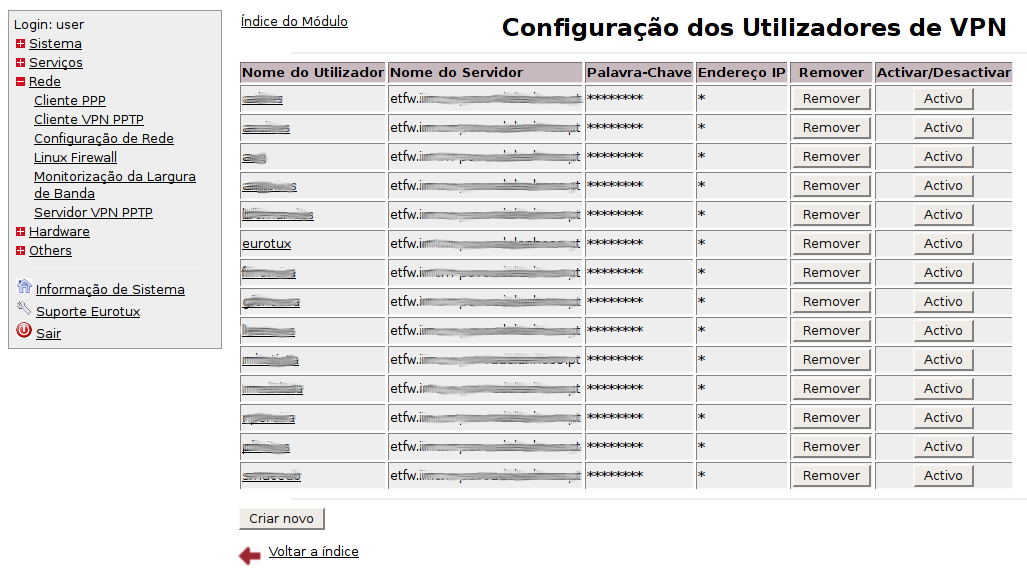
\includegraphics[width=15cm]{../include/img/vpn}
\end{center}
\caption{Edição de utilizadores da VPN}
\label{fig:vpn}
\end{figure}

Este serviço é automaticamente iniciado no arranque da plataforma, mas pode ser desligado utilizando para isso o seguinte comando via SSH ou na linha de comando:

\begin{verbatim}
# service openvpn stop
\end{verbatim}

Pode ser iniciado manualmente através do comando:

\begin{verbatim}
# service openvpn start
\end{verbatim}
